\documentclass[11pt]{book}

\setlength{\oddsidemargin}{0.1in}
\setlength{\evensidemargin}{0.1in}
\setlength{\textwidth}{6.5in}
\setlength{\topmargin}{.04in}
\setlength{\textheight}{8.2in}

%Path to images
\usepackage{graphicx,multicol}
\graphicspath{ {figures/} }
\DeclareGraphicsExtensions{.eps,.png}

%% AMS packages

\usepackage{amsmath,amsfonts,amssymb,amsthm,hhline}

%% other packages
% note that "epstopdf" is required for Mac users

\usepackage{graphics,epstopdf,fancyhdr,palatino, verbatim, bigstrut,
  lscape,enumitem, caption}
\usepackage[abs]{overpic}
\usepackage{graphicx, animate}
\usepackage{color, colortbl}
\definecolor{tracered}{rgb}{1,0.5,0.5}
\definecolor{traceblue}{rgb}{0.5,0.5,1}
\usepackage{makeidx}
\makeindex

\usepackage{hyperref}
\hypersetup{colorlinks=true, linkcolor=blue,  anchorcolor=blue,
citecolor=blue, filecolor=blue, menucolor=blue, pagecolor=blue,
urlcolor=blue,pdftitle={ACmain}}

%% Packages to use the MathDesign _Charter_ font.

%\usepackage[T1]{fontenc}
%\usepackage[charter]{mathdesign}

%% Activities package

% Options to the activities package are: "bighints", "smallhints",
% "activitysolutions" (which are mutually exclusive; the last one listed is the
% one used) "exercisesolutions", and "authornotes".  If the option is there, then
% the corresponding environment is shown.

\usepackage{activities}

\lhead[\fancyplain{}{\thepage}]         {\fancyplain{}{\rightmark}}
\chead[\fancyplain{}{}]                 {\fancyplain{}{}}
\rhead[\fancyplain{}{\rightmark}]       {\fancyplain{\scalebox{0.35}{\includegraphics{figures/CClicense.eps}} }{\thepage}}

\rfoot[\fancyplain{}{}] {\fancyplain{}{\scalebox{0.35}{\includegraphics{figures/CClicense.eps}} }}

\cfoot[\fancyplain{\thepage}{}] {\fancyplain{\thepage}{}}

\lfoot[ \fancyplain{ \scalebox{0.35}{\includegraphics{figures/CClicense.eps}}  }  { \scalebox{0.35}{\includegraphics{figures/CClicense.eps}}  } ] {\fancyplain{}{}}


% \newcounter{cnt}
% \newenvironment{numlist}{\begin{list}{(\arabic{cnt})}{\usecounter{cnt}
% \setlength{\leftmargin}{.35 in}\setlength{\labelwidth}{.35 in}
% \setlength{\itemsep}{10 pt}}}{\end{list}}
\newenvironment{numlist}{\begin{enumerate}[label=(\arabic*),leftmargin=0.35in,labelwidth=0.35in,itemsep=10pt]}{\end{enumerate}}

% \newcounter{cnt4}
% \newenvironment{numlist2}{\begin{list}{(\arabic{cnt4})}{\usecounter{cnt4}
% \setlength{\leftmargin}{.5 in}\setlength{\labelwidth}{.25 in}
% \setlength{\itemsep}{10 pt}}}{\end{list}}
\newenvironment{numlist2}{\begin{enumerate}[label=(\arabic*),leftmargin=0.5in,labelwidth=0.25in,itemsep=10pt]}{\end{enumerate}}

%\newcounter{cnt2}
%\newenvironment{alphalist}{\vspace*{-3 pt}\begin{list}{(\alph{cnt2})}{\usecounter{cnt2}
%\setlength{\leftmargin}{.5 in}\setlength{\labelwidth}{.25
%in}\setlength{\itemsep}{5 pt}}}{\end{list}}
\newenvironment{alphalist}{\vspace*{-3pt}\begin{enumerate}[label=(\alph*),leftmargin=0.5in,labelwidth=0.25in,itemsep=5pt]}{\end{enumerate}}

% \newcounter{cnt3}
% \newenvironment{alphalist2}{\vspace*{-3 pt}\begin{list}{(\alph{cnt3})}{\usecounter{cnt3}
% \setlength{\leftmargin}{.25 in}\setlength{\labelwidth}{.25
% in}\setlength{\itemsep}{5 pt}}}{\end{list}}
\newenvironment{alphalist2}{\vspace*{-3pt}\begin{enumerate}[label=(\alph*),leftmargin=0.25in,labelwidth=0.25in,itemsep=5pt]}{\end{enumerate}}

% \newcounter{cnt5}
% \newenvironment{thmlist}{\vspace*{-3 pt}\begin{list}{{\em (\roman{cnt5})}}{\usecounter{cnt5}
% \setlength{\leftmargin}{.5 in}\setlength{\labelwidth}{.25
% in}\setlength{\itemsep}{3 pt}}}{\end{list}}
\newenvironment{thmlist}{\vspace*{-3pt}\begin{enumerate}[label=\emph{(\roman*)},leftmargin=0.5in,labelwidth=0.25in,itemsep=3pt]}{\end{enumerate}}

%\newcommand{\lint}{\raisebox{-.14 in}{\underline{\hspace*{.7 ex}}}
%\hspace*{-1 ex} \int}

%\newcommand{\uint}{\hspace*{1.5 ex} \raisebox{.296 in}{\underline{\hspace*{.7 ex}}}
%\hspace*{-2.3 ex} \int}

\setlength{\parskip}{5 pt}

\newcounter{lastenum}
\newcommand{\saveCount}{\setcounter{lastenum}{\value{enumi}}}
\newcommand{\restoreCount}{\setcounter{enumi}{\value{lastenum}}}
\newcommand{\addeqno}{\refstepcounter{equation}\tag{\theequation}}

\newcommand{\be}{\begin{numlist}}
\newcommand{\ee}{\end{numlist}}
\newcommand{\bei}{\begin{numlist2}}
\newcommand{\eei}{\end{numlist2}}
\newcommand{\ba}{\begin{alphalist}}
\newcommand{\ea}{\end{alphalist}}
\newcommand{\bal}{\begin{alphalist2}}
\newcommand{\eal}{\end{alphalist2}}
\newcommand{\bi}{\begin{itemize}}
\newcommand{\ei}{\end{itemize}}
\newcommand{\btl}{\begin{thmlist}}
\newcommand{\etl}{\end{thmlist}}


\newcommand{\R}{\mathbb{R}}
\newcommand{\va}{\mathbf{a}}
\newcommand{\vb}{\mathbf{b}}
\newcommand{\vc}{\mathbf{c}}
\newcommand{\vC}{\mathbf{C}}
\newcommand{\vd}{\mathbf{d}}
\newcommand{\ve}{\mathbf{e}}
\newcommand{\vi}{\mathbf{i}}
\newcommand{\vj}{\mathbf{j}}
\newcommand{\vk}{\mathbf{k}}
\newcommand{\vn}{\mathbf{n}}
\newcommand{\vm}{\mathbf{m}}
\newcommand{\vr}{\mathbf{r}}
\newcommand{\vs}{\mathbf{s}}
\newcommand{\vu}{\mathbf{u}}
\newcommand{\vv}{\mathbf{v}}
\newcommand{\vw}{\mathbf{w}}
\newcommand{\vx}{\mathbf{x}}
\newcommand{\vy}{\mathbf{y}}
\newcommand{\vz}{\mathbf{z}}
\newcommand{\vzero}{\mathbf{0}}
\newcommand{\vF}{\mathbf{F}}
\newcommand{\vG}{\mathbf{G}}
\newcommand{\vH}{\mathbf{H}}
\newcommand{\vR}{\mathbf{R}}
\newcommand{\vT}{\mathbf{T}}
\newcommand{\vN}{\mathbf{N}}
\newcommand{\vL}{\mathbf{L}}
\newcommand{\vB}{\mathbf{B}}
\newcommand{\proj}{\text{proj}}
\newcommand{\comp}{\text{comp}}


% theorem-like environments
\theoremstyle{definition}
\newtheorem{pa}{Preview Activity}[chapter]
\newtheorem{example}{Example}[chapter]
\newtheorem{definition}{Definition}[chapter]

\newcommand{\bex}{\begin{center}\underline{\hspace{5.0in}}\end{center} \begin{example}}
\newcommand{\eex}{\end{example} \noindent{\bf Solution.}~~}
\newcommand{\afterex}{\begin{center}\underline{\hspace{5.0in}}\end{center}}
\newcommand{\afterexercises}{\nin \hrulefill \vfill \ \newpage}

% my commands

\newcommand{\ds}{\ensuremath{\displaystyle}}
\newcommand{\nin}{\noindent}
\newcommand{\tr}{\vspace*{0.5in}}
\newcommand{\lr}{\vspace*{1.0in}}
\newcommand{\mr}{\vspace*{2.0in}}
\newcommand{\br}{\vspace*{3.0in}}
\newcommand{\afterpa}{\hfill $\bowtie$}
\newcommand{\aftera}{\hfill $\lhd$}

\newcommand\T{\rule{0pt}{2.6ex}}
\newcommand\B{\rule[-1.2ex]{0pt}{0pt}}

\newenvironment{goals}{ \vspace*{7 pt}{\large \textbf{Motivating Questions}} \vspace*{-6 pt} \\ ~\hrule~ \vspace*{2 pt}

 {\em In this section, we strive to understand the ideas generated by the following important questions:}
\vspace*{-5 pt} \\ ~\hrule~ \vspace*{-3 pt}
\begin{list}{\labelitemi}{\leftmargin=1.25em}
\setlength{\itemsep}{3 pt}}{ \end{list} \vspace*{-2 pt}}

\newenvironment{summary}{ \vspace*{7 pt}
\nin{\large \textbf{Summary}} \vspace*{-6 pt} %\\ ~\hrule~ \vspace*{2 pt}
%\nin{\em \hspace*{-10pt} In this section, we encountered the following important ideas:}
%\vspace*{-9 pt} \\ ~\hrule~ \vspace*{-3 pt}
\begin{list}{\labelitemi}{\leftmargin=1.25em}
\setlength{\itemsep}{3 pt}}{ \end{list} \vspace*{-2 pt}}

\pagestyle{fancyplain}

\setcounter{chapter}{11}

%TABLE/GRAPH ON ONE LINE COMMANDS
%\begin{figure}[h]
%\centering
%\begin{tabular}{cc}
%	\raisebox{.75in}{\begin{tabular}[b]{c|c} $x$ & $y$ \\ \hline a & b \\ c & d \\ e & f  \end{tabular} } &	
%	\hspace{1in} \includegraphics[2in,2in]{c:/mth310/project/Hamilton.bmp}
%\end{tabular}
%\caption{{\scriptsize Table and graph for $f$.}}
%\end{figure}

%%%%%%%%%%%%%%%%%%%%%%%%%%%%%%%%%%%%%%%%%%%%%%%%%%%%

\title{Active Calculus - Multivariable \\ \vspace{0.02in} \small{2015 edition} \\ \vspace{0.1in} \scalebox{0.75}{\includegraphics{figures/CClicense.eps}}}
%\date{\today}
\author{Steve Schlicker, Lead Author and Editor \\ Department of Mathematics \\ Grand Valley State University \\
\texttt{schlicks@gvsu.edu} \\
\href{http://faculty.gvsu.edu/schlicks/}{\texttt{http://faculty.gvsu.edu/schlicks/}}\\
\vspace{1.5in} \\
David Austin, Contributing Author \\
\href{http://merganser.math.gvsu.edu/david/}{\texttt{http://merganser.math.gvsu.edu/david/}} \\ \ \\
Matt Boelkins, Contributing Author \\
\href{http://faculty.gvsu.edu/boelkinm/}{\texttt{http://faculty.gvsu.edu/boelkinm/}} }

%\includeonly{6.chap}

\begin{document}
\frontmatter
\maketitle
\tableofcontents


\mainmatter

\chapter{Vector Calculus} \label{C:12}

\section{Vector Fields} \label{S:12.1.VectorFields}


\vspace*{-14 pt}
\framebox{\hspace*{3 pt}
\parbox{6.25 in}{\begin{goals}
\item What is a vector field?
\item How do we draw a vector field?
\item What are some familiar contexts in which vector fields arise?
\end{goals}} \hspace*{3 pt}}

\subsection*{Introduction}

Thus far vectors have played a central role in our study of
multivariable calculus. We know how to do operations on vectors
(addition, scalar multiplication, dot product, etc.), and we have seen
how vectors can be used to describe curves in $\R^2$ and $\R^3$. The
examples of using vectors to describe curves was our first example of
a vector-valued function. That is, a curve $\vr(t)$ is really a
function that takes as input a real number and produces a vector in
$\R^2$ or $\R^3$. In this section we will expand our understanding of
vector-valued functions to take as input a point $(x,y)$ in $\R^2$ or
a point $(x,y,z)$ in $\R^3$ and produce a vector (typically in $\R^2$
or $\R^3$, respectively).


\begin{pa} \label{PA:12.1}
It's common for weather forecasters to discuss the wind \emph{speed}, but as any student who has gotten this far in the text will know, this nomenclature is imprecise. It's not terribly helpful to tell someone the wind is blowing at $10$ km/h without telling them the direction in which the wind is blowing. If you're trying to make a decision based on what the wind is doing, you need to know about the direction as well. (Perhaps you are taking off in a hot air balloon and need to know which direction the chase team should head to keep track of you.) Because of the swirling nature of wind, it makes sense to give the wind \emph{velocity} at every point in a region (two-dimensional or three-dimensional). 

\ba
\item \label{enum:PA12.1F} Suppose that given a point $(x,y)$ in the plane, you know that the wind velocity at that point is given by the vector $\vF(x,y) = \langle y,x\rangle$. For example, we'd then know that at the point $(1,-1)$, the wind velocity is $\vF(1,-1) = \langle -1,1\rangle$. In the table below, fill in the wind velocity vectors for the given points.
  \begin{center}
    \begin{tabular}{c|c|c|c|c|c}
      $(x,y)$ & $(2,1)$ & $(0,0)$ & $(-1,2)$ & $(3,-1)$ & $(-2,-1)$\\\hline
$\vF(x,y)$ & & & & &
    \end{tabular}
  \end{center}
\item \label{enum:PA12.1G} Suppose that we associate the vector $\vG(x,y) = -x\vj$ to a point $(x,y)$ in the plane. Complete the table below by giving the vector associated to each of the given points.
  \begin{center}
    \begin{tabular}{c|c|c|c|c|c|c|c|c}
      $(x,y)$ & $(-2,0)$ & $(-1,2)$ & $(0,-2)$ & $(1,1)$ & $(2,3)$ & $(3,2)$ & $(-1,0)$ & $(1,3)$\\\hline
$\vG(x,y)$ & & & & & & &
    \end{tabular}
  \end{center}

\saveCount
\ea

A table of values of these vector-valued functions is useful, but perhaps even better is a method of visualizing the vectors. In keeping with our wind velocity analogy, if $\vF(2,1) = \langle 1,2\rangle$, we draw the vector $\langle 1,2\rangle$ with its tail at the point $(2,1)$. 

\ba
\restoreCount
\item Using the first set of axes in Figure~\ref{fig:PA12.1a}, plot the vectors $\vF(x,y)$ for the five points in the table in part \ref{enum:PA12.1F}. The example $\vF(1,-1) = \langle -1,1\rangle$ is drawn for you.
\item Using the second set of axes in Figure~\ref{fig:PA12.1a}, plot the vectors $\vG(x,y)$ for the eight points in the table in part \ref{enum:PA12.1G}. 
% TODO: Actually include the promised vector on the left grid.
  \begin{figure}[h]
    \centering
    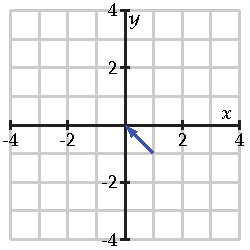
\includegraphics{figures/PA12-1F-axes.pdf}\hspace{0.5in}    \includegraphics{figures/PA12-1G-axes.pdf}
    \caption{Axes for plotting some vectors from $\vF(x,y)$ and $\vG(x,y)$.}
    \label{fig:PA12.1a}
  \end{figure}
\ea
\end{pa} 
\afterpa 
%%% Local Variables:
%%% mode: latex
%%% TeX-master: "../0_AC_MV"
%%% End:


\subsection*{Examples of Vector Fields}

As Preview Activity~\ref{PA:12.1} showed you, one example of a time
where it makes sense to associate a vector to each point in a region
is a \emph{velocity vector field} $\vF(x,y)$ or $\vF(x,y,z)$, where
the vector associated to the point $(x,y)$ or $(x,y,z)$ is the
velocity of something at that point. Wind velocity is one example, but
another example would be the velocity of a flowing fluid.
Figure~\ref{fig:12.1.fluid-velocity} shows such a velocity vector
field. Technically, it only shows some of the vectors in the vector
field, since the figure would be unintelligible if all of the vectors
were shown. This is illustrated by the inset in the upper left corner,
which gives a better picture of what we would see if we zoomed in on
the red square of the main figure.

\begin{figure}[h]
  \centering
  \includegraphics[width=0.9\linewidth]{figures/12_1_PIVlab_multipass.jpg}

  \vspace{-5pt}{\scriptsize \href{https://commons.wikimedia.org/wiki/File:PIVlab_multipass.jpg\#/media/File:PIVlab_multipass.jpg}{"PIVlab multipass" by Willa} - Own work. Licensed under CC-BY-SA 3.0 via Wikimedia Commons}
  \caption{An illustration of some of the vectors in a fluid velocity
    vector field.}
  \label{fig:12.1.fluid-velocity}
\end{figure}

Force fields, such as those created by gravity, are also examples of
vector fields. For example, the earth exerts a gravitational force on
objects. The force is directed from the center of the object to the
center of the earth, and its magnitude is determined by the distance
between the object and the earth. An illustration of this vector field
can be seen in Figure~\ref{fig:12.1.gravity}, where the earth is
positioned at the origin, but not shown. Notice that the vectors get
shorter as the distance from the origin increases, reflecting the fact
that the gravitational force is weaker at that distance.

\begin{figure}[h]
  \centering
  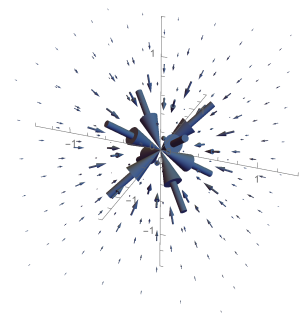
\includegraphics[width=0.4\linewidth]{figures/12_1_gravity_field.pdf}
  \caption{Gravitational vector field.}
  \label{fig:12.1.gravity}
\end{figure}

\subsection*{Mathematical Vector Fields}

As suggested in the introduction and Preview Activity~\ref{PA:12.1},
vector fields can be given by formulas.

\vspace*{5pt}
\nin \framebox{\hspace*{3 pt}
  \parbox{6.25 in}{\begin{definition} A
      \textbf{vector field}\index{vectorfield!definition} in $2$-space
      function whose value at a point $(x,y)$ is a $2$-dimensional
      vector $\vF(x,y)$. In $3$-space, a vector field is similarly a
      function $\vF(x,y,z)$ whose value at the point $(x,y,z)$ is a
      $3$-dimensional vector.
\end{definition} } \hspace*{3 pt}} \vspace*{5pt}

Since $\vF(x,y,z)$ is a vector, it has $\vi$, $\vj$, and $\vk$
components. Each of these components is a scalar function of the point
$(x,y,z)$, and so we will often write
\[\vF(x,y,z) = F_1(x,y,z)\vi + F_2(x,y,z)\vj + F_3(x,y,z)\vk.\]
For example, if $\vF(x,y,z) = \langle x^2,xy\sin(z),y^3\rangle$, then
$F_1(x,y,z) = x^2$, $F_2(x,y,z) = xy\sin(z)$, and $F_3(x,y,z) =
y^3$. Any time we are considering a vector field $\vF(x,y,z)$, the
definitions of functions $F_1$, $F_2$, and $F_3$ should be assumed in
this manner. (For a vector field $\vF(x,y)$ in $2$-space, we only have
the functions $F_1$ and $F_2$, defined analogously.)

\subsection*{Plotting Vector Fields}

Preview Activity~\ref{PA:12.1} gave you a chance to plot some vectors
in the vector fields $\vF(x,y) = \langle y,x\rangle$ and $\vG(x,y) =
\langle 0,-x\rangle$. It would be impossible to sketch \emph{all} of
the vectors in these vector fields, since there is one for every point
in the plane. In fact, even sketching by hand many more of the vectors
than you were asked to in the preview activity rapidly becomes
tedious. Fortunately, computer algebra systems can do a great job of
making such sketches. One thing to keep in mind, however, is that the
magnitudes of the vectors are typically scaled in these plots,
including plots of vector fields we will encounter later in the
text. To illustrate this, consider the two plots of the vector field
$\vF(x,y) = y\vi + x\vj$ in Figure~\ref{fig:12.1.scale-field}. 
\begin{figure}[h]
  \centering
  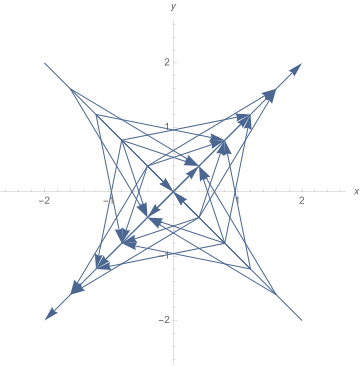
\includegraphics[width=0.3\linewidth]{figures/12_1_vecfield_unscaled.pdf}\hspace{0.2\linewidth}  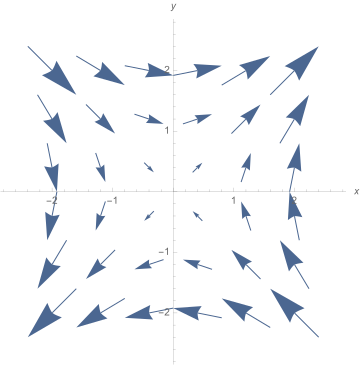
\includegraphics[width=0.3\linewidth]{figures/12_1_vecfield_scaled.pdf}
  \caption{Two plots of $\vF(x,y) = y\vi + x\vj$ from a computer
    algebra system}
  \label{fig:12.1.scale-field}
\end{figure}
The left plot shows some of the vectors but accurately depicts all of
their magnitudes, making the figure very hard to understand,
especially along the lines $y=x$ and $y=-x$. The plot on the right,
however, uses a uniform scaling to make the figure easier to read. As
before, each vector's direction is completely accurate, but now the
magnitudes are much smaller. However, the \emph{relative} magnitudes
are preserved, helping us to see that vectors farther from the origin
have larger magnitude than those closer to the origin.


\begin{activity} \label{A:12.1.1}  
\nin The plot in Figure~\ref{fig:12.1.circle} illustrates the vector
field $\vF(x,y) = y\vi -x\vj$.
\begin{figure}[h]
  \centering
  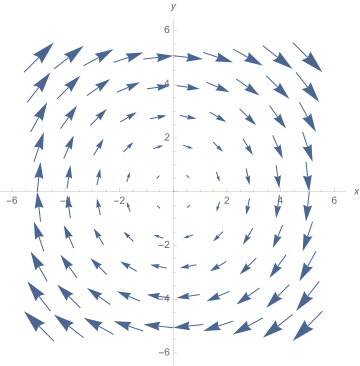
\includegraphics[width=0.35\linewidth]{12_1_circle.pdf}
  \caption{The vector field $y\vi-x\vj$}
  \label{fig:12.1.circle}
\end{figure}
\ba
\item Starting with one of the vectors near the point $(2,0)$, sketch
  a curve that follows the direction of the vector field $\vF$. To
  help visualize what you are doing, it may be useful to think of the
  vector field as the velocity vector field for some flowing water and
  that you are imagining tracing the path that a tiny particle
  inserted into the water would follow as the water moved it around.
\item Repeat the previous step for at least two other starting points
  not on the curve you previously sketched.
\item What shape do the curves you sketched in the previous two steps
  form?
\item Verify that $\vF(x,y)$ is orthogonal to $\langle x,y\rangle$.
\item What is the relationship between the function $f(x,y) = x^2 +
  y^2$ and the vector $x\vi + y\vj$? %(You might find it useful to
%  think about the vector $2x\vi + 2y\vj$ first.) 
\item What does this tell you about the relationship between
  $\vF(x,y)$ and circles centered at the origin?  What is the
  relationship between $|\vF(x,y)|$ and the radius of the appropriate circle?
\ea
\end{activity}
\begin{smallhint}

\end{smallhint}
\begin{bighint}

\end{bighint}
\begin{activitySolution}

\end{activitySolution}
\aftera
%%% Local Variables:
%%% mode: latex
%%% TeX-master: "../0_AC_MV"
%%% End:


\subsection*{Gradient Vector Fields}

Without using the terminology, we've actually already encountered one
very important family of vector fields a number of times. Given a function $f$ of two or three variables, the gradient of
$f$ is a vector field, since for any point where $f$ has first-order
partial derivatives, $\nabla f$ assigns a vector to that point.

\begin{activity} \label{A:12.1.2}  
\ba
\item In Figure~\ref{fig:12.1.level-curves} there are three sets of axes showing level
  curves for functions $f$, $g$, and $h$, respectively. Sketch at least six vectors
  in the gradient vector field for each function. In making your
  sketches, you don't have to worry about getting vector magnitudes
  precise, but you should ensure that the relative magnitudes (and directions) are
  correct for each function independently.
  \begin{figure}[h]
    \centering
    \parbox[t]{0.3\linewidth}{\centering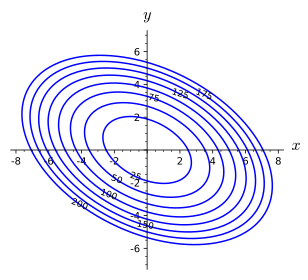
\includegraphics[width=\linewidth]{../figures/12_1_ellipses.pdf}\\\hspace{-4pt}$f$}\hspace{0.04\linewidth}\parbox[t]{0.3\linewidth}{\centering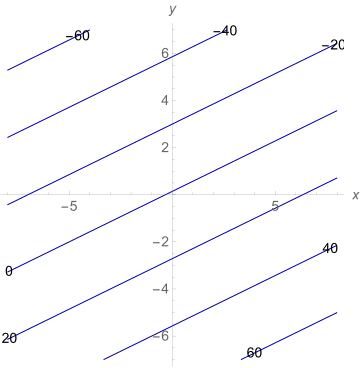
\includegraphics[width=\linewidth]{../figures/12_1_linear.pdf}\\\hspace{-4pt}$g$}\hspace{0.04\linewidth}\parbox[t]{0.3\linewidth}{\centering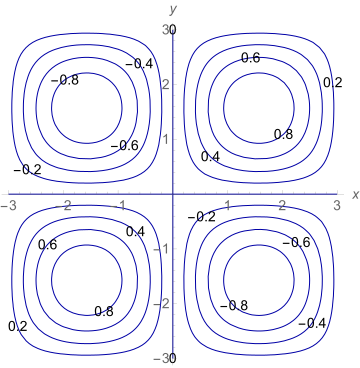
\includegraphics[width=\linewidth]{../figures/12_1_sine.pdf}\\\hspace{-3pt}$h$}
    \caption{Three sets of level curves}
    \label{fig:12.1.level-curves}
  \end{figure}
\item Verify that $\vF(x,y) = \langle 6xy,3x^2+9\sqrt{y}\rangle$ is a
  gradient vector field by finding a function $f$ such that $\nabla
  f(x,y) = \vF(x,y)$. For reasons originating in physics, such a
  function $f$ is called a \emph{potential function} for the vector
  field $\vF$.\label{part:A12.2-pot}
\item Is the function $f$ found in part \ref{part:A12.2-pot} unique?
  That is, can you find another function $g$ such that $\nabla g(x,y)
  = \vF(x,y)$ but $f\neq g$?
\item Is the vector field $\vF(x,y) = 6xy\vi +(2x+9\sqrt{y})\vj$ a
  gradient vector field? Why or why not?
\ea
\end{activity}
\begin{smallhint}

\end{smallhint}
\begin{bighint}

\end{bighint}
\begin{activitySolution}

\end{activitySolution}
\aftera
%%% Local Variables:
%%% mode: latex
%%% TeX-master: "../0_AC_MV"
%%% End:



%\nin \framebox{\hspace*{3 pt}
%\parbox{6.25 in}{
\begin{summary}
\item A $2$-dimensional vector field is a function defined on part of
  $\R^2$ whose value is a $2$-dimensional vector. A $3$-dimensional
  vector field is a function defined on part of $\R^3$ whose value is
  a $3$-dimensional vector.
\item Vector fields arise in familiar contexts such as wind velocity,
  fluid velocity, and gravitational force.
\item Vector fields are generally plotted in ways that ensure the
  direction and relative magnitudes of the vectors sketched are
  correct instead of ensuring that each vector's magnitude is
  depicted correctly.
\item The gradient of a function $f$ of two or three variables is a vector
  field defined wherever $f$ has partial derivatives.
\end{summary}
%} \hspace*{3 pt}}

\nin \hrulefill

%\input{exercises/9.2.Vectors(Ex)}

\clearpage

%%% Local Variables:
%%% mode: latex
%%% TeX-master: "0_AC_MV"
%%% End:

\section{The Idea of a Line Integral} \label{S:12.2.IdeaLineIntegral}


\vspace*{-14 pt}
\framebox{\hspace*{3 pt}
\parbox{6.25 in}{\begin{goals}
\item What is a line integral of a vector-valued function along a curve?
\item How can we estimate if a line integral of a vector-valued
  function along a curve is positive, negative, or zero?
\end{goals}} \hspace*{3 pt}}

\subsection*{Introduction}

As we discussed in section \ref{S:12.1.VectorFields}, vector fields
are often useful as representations of forces such as gravity, wind,
and flowing water. We learned in section \ref{S:9.3.Dot_Product} that
the dot product of a force vector and a displacement vector tells us
how much work the force did on the object as it moved from the tail of
its displacement vector to the tip. However, things more complicated
when an object's movement is not in a straight line and when the force
is not uniform throughout the area in which the object moves. For
example, how much work does a wind of $30$ mph toward the northwest do
on an airplane that's flying 500 miles due north? What if the wind
gets weaker the farther north the plane gets? In this
section, we begin investigating how integration can be used to
calculate the work a force field does in such circumstances.

\begin{pa} \label{PA:12.2}
Recall from Section~\ref{S:9.3.Dot_Product} that the work done by a
force $\vF$ on an object that moves with displacement vector $\vv$ is
$\vF\cdot \vv$. In this Preview Activity, we will consider the work
done by a wind blowing due east at $45$ miles per hour on an airplane
at various stages of its journey.
\ba
\item A pilot flies for an hour and finds that he is $300$ miles from
  where he started at a heading of $20^\circ$ degrees east of due
  north. Find the work the wind has done on the airplane during the
  flight.
\item An hour later, the pilot determines that he is $275$ miles due
  north of where he previously checked his position. Find the work
  done by the wind on the airplane during the second hour of the
  flight.
\item Find the pilot's displacement from his original position after
  two hours of flying and use that to find the work done by the wind
  on the airplane during the first two hours of flight.
\item How does your answer to the previous part connect to the answers
  to the first two parts?
\item Suppose that the pilot then flies $45^\circ$ west of due north
  for $200$ miles. Find the work done by the wind on the airplane
  during this part of the journey.
\ea
\end{pa} 
\afterpa 
%%% Local Variables:
%%% mode: latex
%%% TeX-master: "../0_AC_MV"
%%% End:


\subsection*{Orientations of Curves}

Given our motivation for calculating the work that a force field does
on an object as it moves through the field, it is natural to concern
ourselves with \emph{how} the object moves. In particular, in many
circumstances it will be different if an object moves from the point
$(0,1)$ to the point $(4,3)$ by first going up the $y$-axis to $(0,3)$
and then moving horizontally to $(4,3)$ than if the object moves along
the line segment from $(0,1)$ directly to $(4,3)$. Similarly, given a
fixed force field, we would expect the work done to be different (in
fact, opposite) if the object moves from $(4,3)$ to $(0,1)$ directly
along a line segment. We say that a curve in $\R^2$ or $\R^3$ is
\emph{oriented} if we have specified the direction of travel along the
curve. When a curve is given parametrically (including as a
vector-valued function), our convention will be that the orientation
follows from the smallest allowable value of the parameter to the largest.


\begin{activity} \label{A:12.2.1}  
\nin Find parameterizations of each of the curves described
below. Ensure that each curve's orientation matches the one specified.
\ba
\item The line segment in $\R^3$ from $(0,1,-2)$ to $(3,-1,2)$.
\item The line segment in $\R^3$ from $(3,-1,2)$ to $(0,1,-2)$.
\item The circle of radius $3$ (in $\R^2$) centered at the origin,
  beginning at the point $(0,-3)$ and proceeding clockwise around the
  circle.
\item The portion of the parabola $y^2 = x$ from the point $(4,2)$ to
  the point $(1,-1)$.
\ea
\end{activity}
\begin{smallhint}

\end{smallhint}
\begin{bighint}

\end{bighint}
\begin{activitySolution}

\end{activitySolution}
\aftera
%%% Local Variables:
%%% mode: latex
%%% TeX-master: "../0_AC_MV"
%%% End:


\subsection*{Line Integrals}

Just as when we differentiated a vector-valued function $\vr(t)$ to
find a tangent vector, we begin by dividing a curve $C$ oriented from
a point $P$ to a point $Q$ into $n$ small, straight pieces. Each of
these pieces is in an area where the vector field $\vF$ is nearly
constant. In Figure~\ref{fig:12.2.curve-vectors}, we show this
situation. Each $\vr_i$ is the tip of a vector that traces out the
curve, and then the $\Delta\vr_i = \vr_{i+1}-\vr_i$ (shown in blue)
approximate the curve $C$. The green vectors are the vectors in the
vector field $\vF$ at each of the designated points along the curve.

\begin{figure}[h]
  \centering
  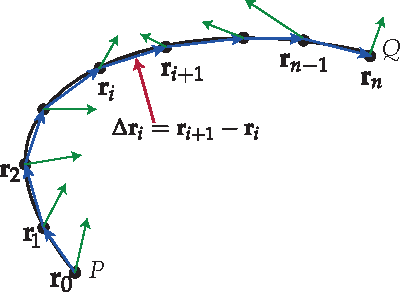
\includegraphics[width=0.45\linewidth]{figures/fig_12_2_curve_vec_field.pdf}
  \caption{A curve $C$ oriented from the point $P$ to the point
    $Q$. The tips of the vectors $\vr_i$ that trace out the curve are
    shown as points. The blue vectors are the $\Delta\vr_i$, while the
  green vectors are the vectors associated to each of the points by a
  vector field $\vF$.}
  \label{fig:12.2.curve-vectors}
\end{figure}

If we are trying to figure out how much a wind current helps or
hinders an aircraft flying along a path determined by the curve, then
calculating the dot product $\vF(\vr_i)\cdot \Delta\vr_i$ makes sense for
the local amount of help/hindrance, as if the vector $\vr_i$ along the
curve and the force field vector $\vF(\vr_i)$ point in similar
directions, the dot product will be positive.\footnote{We are abusing
  notation here a tiny bit, since technically the domain of $\vF$ is
  points in $\R^2$ or $\R^3$, and $\vr_i$ is a vector. By $\vF(\vr)$,
  we mean $\vF(r_1,r_2)$, where $\vr= \langle r_1,r_2\rangle$.} On the other hand, if
the angle between them is obtuse, the dot product will be negative and
we also would note that the force field is hindering the aircraft's
progress. Taking the sum over $i=0,\dots,n-1$, we have a Riemann sum
that approximates the work done by the vector field on the aircraft as
it flies along $C$:
\[\sum_{i=0}^{n-1}\vF(\vr_i)\cdot\Delta \vr_i.\]
This suggests the following definition.

\vspace*{5pt}
\nin \framebox{\hspace*{3 pt}
  \parbox{6.25 in}{\begin{definition} \label{def:12.2.line-integral}Let $C$ be an oriented curve and
      $\vF$ a vector field defined in a region containing $C$. The
      \textbf{line integral}\index{lineintegral!definition} of $\vF$
      along $C$ is
      \[\int_C \vF\cdot d\vr = \lim_{|\Delta\vr_i|\to 0}
      \sum_{i=0}^{n-1}\vF(\vr_i)\cdot\Delta\vr_i,\]
      provided the limit exists.
\end{definition} } \hspace*{3 pt}} \vspace*{5pt}

The limit in definition~\ref{def:12.2.line-integral} exists provided
that $\vF$ is a continuous vector field, by which we mean that each
component function of $\vF$ is continuous as a function of $2$ or $3$
variables, and that $C$ is a piecewise smooth curved traced out from
its initial point to its terminal point without retracing any portion
of the curve.

Because the dot products in the definition of the line integral
$\int_C\vF\cdot d\vr$ can each be viewed as the work done by $\vF$ as
an object moves along the (very small) vector $\Delta\vr$, the line
integral gives the total work done by the vector field on an object
that moves along $C$ (in the direction of its orientation).

\begin{activity} \label{A:12.2.2} \nin Shown in
  Figure~\ref{F:12.2-idea-figs} are two vector fields, $\vF$ and $\vG$
  and four oriented curves, as labeled in the plots. For each of the
  line integrals below, determine if its value should be positive,
  negative, or zero.
  \begin{multicols}{4}
\begin{enumerate}[label=(\alph*)]
  \item $\int_{C_1}\vF\cdot d\vr$
  \item $\int_{C_2}\vF\cdot d\vr$
  \item $\int_{C_3}\vG\cdot d\vr$
  \item $\int_{C_4}\vG\cdot d\vr$ 
\end{enumerate}
  \end{multicols}
\begin{figure}[h]
  \centering
  \begin{overpic}[width=0.45\linewidth]{figures/fig_12_2_idea_field_1.pdf}\put(110,100){$C_1$}\put(125,50){$C_2$}\end{overpic}\hspace{0.05\linewidth}  \begin{overpic}[width=0.45\linewidth]{figures/fig_12_2_idea_field_2.pdf}\put(85,173){$C_3$}\put(125,50){$C_4$}\end{overpic}
  \caption{Vector fields $\vF$ (left) and $\vG$ (right)}\label{F:12.2-idea-figs}
\end{figure} 
\end{activity}
\begin{smallhint}

\end{smallhint}
\begin{bighint}

\end{bighint}
\begin{activitySolution}

\end{activitySolution}
\aftera
%%% Local Variables:
%%% mode: latex
%%% TeX-master: "../0_AC_MV"
%%% End:


The next several sections will be devoted to determining ways to
calculate line integrals, since the limit in the definition, just like
the limit in the definition of every other type of integral we've
studied so far, is cumbersome to work with in most cases. However, in
the case where the oriented curve $C$ is composed of horizontal and
vertical line segments, we can make a rather quick reduction to a
single-variable integral, as the following example shows.

\begin{example}\label{ex:12.2.line-int}
  Consider the constant vector field $\vF(x,y) = \langle
  2,1\rangle$. Let $C$ be the curve that follows the horizontal line
  segment from $(1,1)$ to $(4,1)$ and then continues down the vertical
  line segment to $(4,-2)$. Figure~\ref{fig:12.2.curve-field} shows
  $\vF$ and $C$, including the orientation.

\begin{figure}[h]
  \centering
  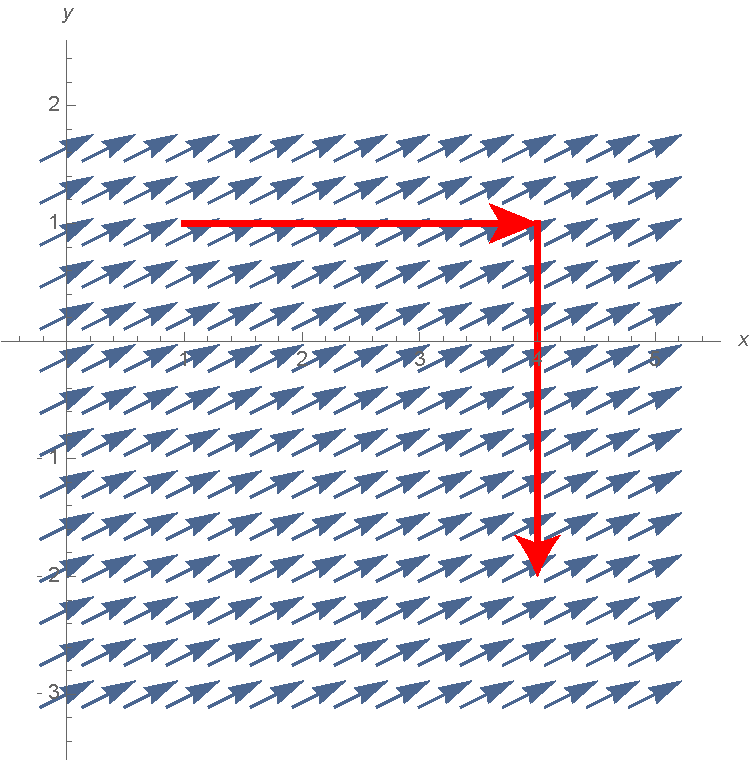
\includegraphics[width=0.45\linewidth]{figures/fig_12_2_field_line_segs.pdf}
  \caption{An oriented curve from $(1,1)$ to $(4,-2)$ in a vector
    field $\vF$.}
  \label{fig:12.2.curve-field}
\end{figure}

To calculate $\int_C\vF\cdot d\vr$, we'll start by working with the
horizontal line segment. Along that part of $C$, notice that
$d\vr\approx \Delta\vr = \Delta x\vi$. Thus, the Riemann sum that
calculates the line integral along this portion of $C$ consists of
terms of the form $\langle 2,1\rangle\cdot (\Delta x \vi) = 2\Delta
x$. Along this part of $C$, $x$ ranges from $1$ to $4$, and thus we
can turn the Riemann sum here into the definite integral $\int_1^4 2\,
dx = 6$. Since the vectors are generally pointing in a direction that
agrees with the orientation of $C$, we are not surprised to have a
positive value here.

Now we turn our attention to the vertical portion of $C$. Here $d\vr
\approx \Delta\vr = \Delta y\vj$, which means that $\vF\cdot
d\vr\approx 1\Delta y$. Hence, our Riemann sum can
be calculated by the definite integral $\int_1^{-2} 1\, dy =
-3$. Notice that the limits of integration here were set up to match
the orientation of $C$. Also, the negative value should not be
unexpected, since $C$ is oriented in a direction for which the vectors
of $\vF$ point in a direction that would hinder motion along $C$.

Combining these two pieces of work, we find that $\int_C \vF\cdot d\vr
= 6 - 3 = 3$.
\end{example}

\subsection*{Properties of Line Integrals}

In Example~\ref{ex:12.2.line-int}, we implicitly made use of the idea
that if $C$ can be broken up into two curves $C_1$ and $C_2$ such that
the endpoint of $C_1$ is the start point of $C_2$, then the line
integral of $\vF$ along $C$ is the sum of the line integrals of $\vF$
along $C_1$ and along $C_2$. This probably seems natural, based on the
property for definite integrals which tells us that
\[\int_a^b f(x)\, dx = \int_a^c f(x)\, dx + \int_c^b f(x)\, dx.\]
The table below summarizes some other properties of line integrals,
each of which has a familiar analogue amongst the properties of
definite integrals. If $C_1$ and $C_2$ are oriented curves, with $C_1$
from a point $P$ to a point $Q$ and $C_2$ from $Q$ to a point $R$, we
denote by $C_1+C_2$ the oriented curve from $P$ to $R$ that follows
$C_1$ to $Q$ and then continues along $C_2$ to $R$. Also, if $C$ is an
oriented curve, $-C$ denotes the same curve but with the opposite
orientation.


\vspace*{5pt}
\nin 
\framebox{
  \hspace*{3 pt}
  \parbox{6.25 in}{
    For a constant scalar $k$, vector fields $\vF$ and $\vG$, and
    oriented curves $C$, $C_1$, and $C_2$, the following properties hold:
    \begin{enumerate}
    \item $\ds\int_C (k\vF)\cdot d\vr = k\int_C\vF\cdot d\vr$
    \item $\ds\int_C(\vF+\vG)\cdot d\vr = \int_C \vF\cdot d\vr +
      \int_C\vG\cdot d\vr$
    \item $\ds\int_{-C}\vF\cdot d\vr = -\int_C \vF\cdot d\vr$
    \item $\ds\int_{C_1+C_2} \vF\cdot d\vr = \int_{C_1}\vF\cdot d\vr +
      \int_{C_2}\vF\cdot d\vr$.
    \end{enumerate}
  } 
  \hspace*{3 pt}
}
\vspace*{5pt}

\begin{activity} \label{A:12.2.3}  

\nin Figure~\ref{F:12.2-field-practice} shows a vector field $\vF$ as
well as six oriented curves, as labeled in the plot.
\begin{figure}[h]
  \centering
  \begin{overpic}[width=0.55\linewidth]{figures/fig_12_2_field_practice.pdf}
    \put(140,55){$C_5$}
    \put(50,130){$C_6$}
    \put(169,135){$C_1$}
    \put(190,183){$C_2$}
    \put(170,230){$C_3$}
    \put(131,184){$C_4$}
  \end{overpic}
  \caption{A vector field $\vF$ and six oriented curves.}\label{F:12.2-field-practice}
\end{figure} 
\ba
\item Is $\int_{C_5}\vF\cdot d\vr$ positive, negative, or zero? Explain.
\item Let $C = C_1+C_2+C_3+C_4$. Determine if $\int_C\vF\cdot d\vr$ is
  positive, negative, or zero.
\item Order the line integrals below from smallest to largest.
\[\int_{C_1}\vF\cdot d\vr\qquad \int_{C_2}\vF\cdot d\vr\qquad \int_{C_3}\vF\cdot d\vr\qquad \int_{C_4}\vF\cdot d\vr\qquad \int_{C_5}\vF\cdot d\vr\qquad \int_{C_6}\vF\cdot d\vr\]
\ea
\end{activity}
\begin{smallhint}

\end{smallhint}
\begin{bighint}

\end{bighint}
\begin{activitySolution}

\end{activitySolution}
\aftera
%%% Local Variables:
%%% mode: latex
%%% TeX-master: "../0_AC_MV"
%%% End:


\subsection*{The Circulation of a Vector Field}

If an oriented curve $C$ ends at the same point where it started, we
say that $C$ is \textbf{closed}. The line integral of a vector field
$\vF$ along a closed curve $C$ is called the \textbf{circulation} of
$\vF$ around $C$. To emphasize the fact that $C$ is closed, we
sometimes write $\oint_C \vF\cdot d\vr$ for $\int_C \vF\cdot
d\vr$. Circulation servies as a measure of a vector field's tendency
to rotate in a manner consistent with the orientation of the curve.

\begin{activity} \label{A:12.2.4}  
\nin Determine if the circulation of the vector field around each of the
closed curves shown in Figure~\ref{F:12.2-circ} below is positive, negative, or zero.
\begin{figure}[h]
  \centering
  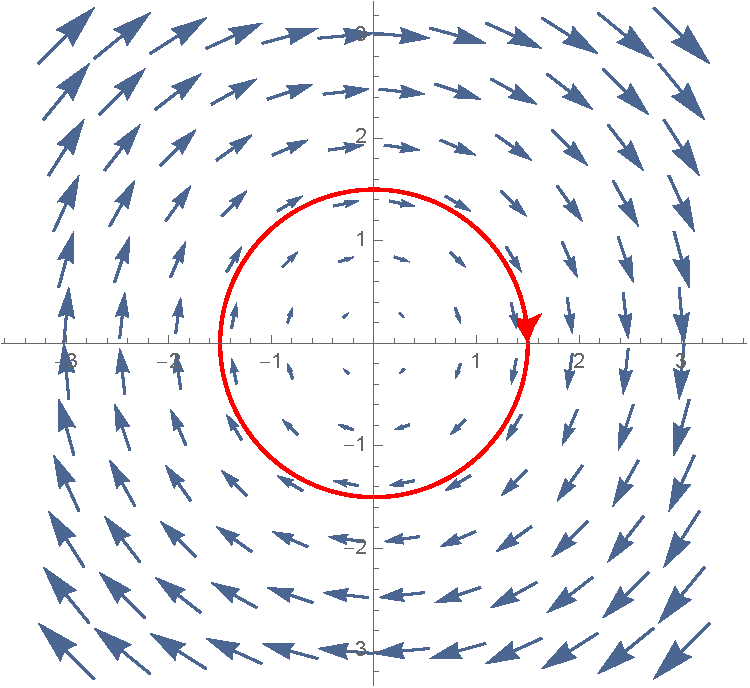
\includegraphics[width=0.45\linewidth]{figures/fig_12_2_circ_circle.pdf}  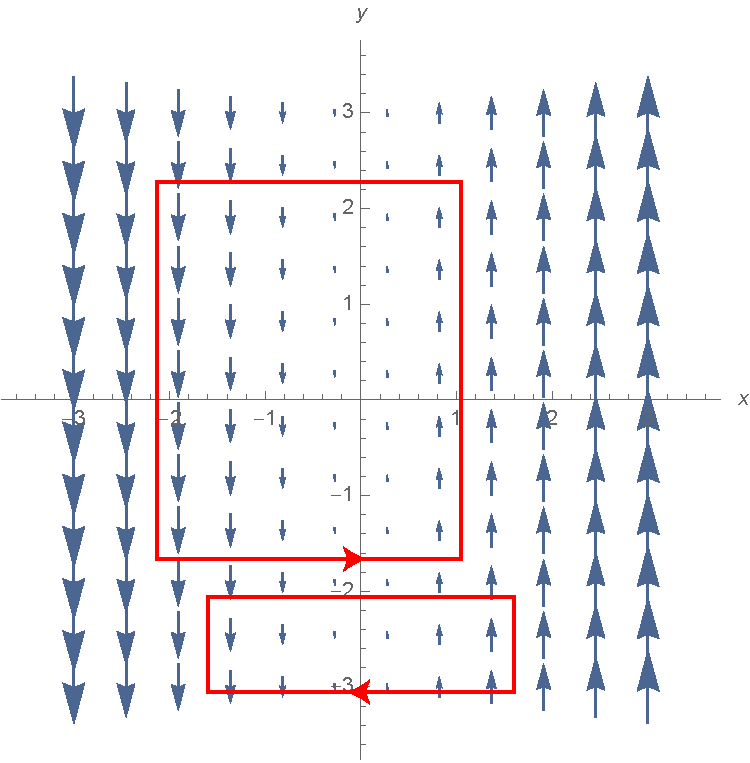
\includegraphics[width=0.45\linewidth]{figures/fig_12_2_circ_box.pdf}
  \caption{Vector fields and closed curves}\label{F:12.2-circ}
\end{figure} 
\end{activity}
\begin{smallhint}

\end{smallhint}
\begin{bighint}

\end{bighint}
\begin{activitySolution}

\end{activitySolution}
\aftera
%%% Local Variables:
%%% mode: latex
%%% TeX-master: "../0_AC_MV"
%%% End:

% In Figure~\ref{fig:12.2.circulation}

% \begin{figure}[h]
%   \centering
%   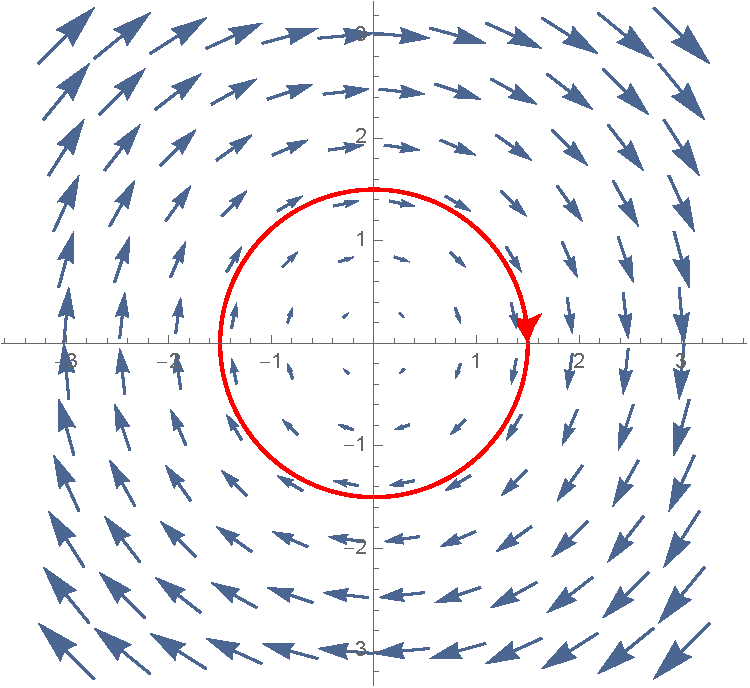
\includegraphics[width=0.45\linewidth]{figures/fig_12_2_circ_circle.pdf}  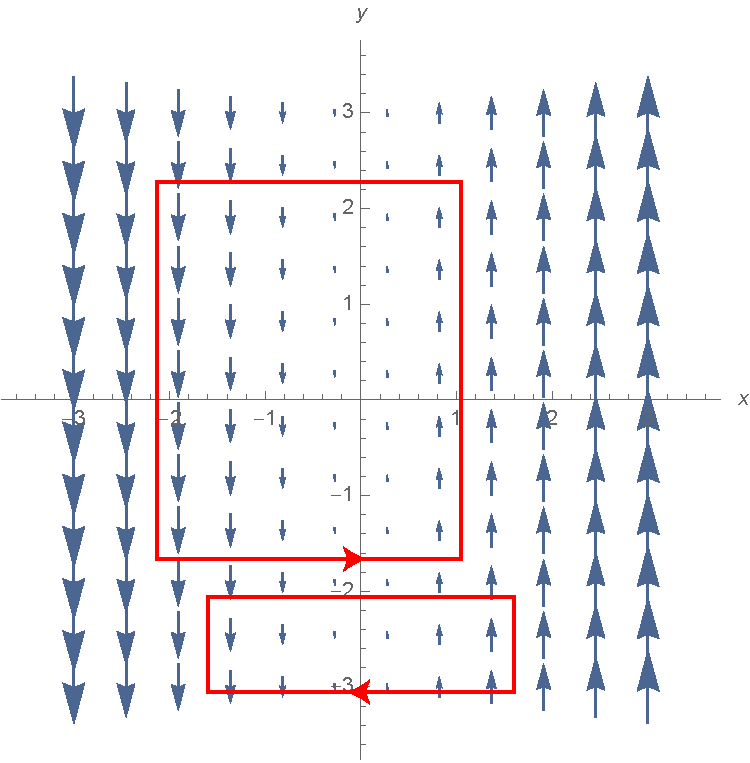
\includegraphics[width=0.45\linewidth]{figures/fig_12_2_circ_box.pdf}

%   \caption{Closed oriented curves in vector fields}
%   \label{fig:12.2.curve-vectors}
% \end{figure}


%\nin \framebox{\hspace*{3 pt}
%\parbox{6.25 in}{
\begin{summary}
\item A line integral measures of a vector field along an oriented
  curve measures the extent to which the vector field points in a
  direction consistent with the orientation of the curve.
\item Line integrals are defined using Riemann sums by breaking the
  curve into many small segments along which the vector field is
  essentially constant.
\item Line integrals have many properties that are analogous to those
  of definite integrals of functions of a single variable.
\end{summary}
%} \hspace*{3 pt}}

\nin \hrulefill

%\input{exercises/9.2.Vectors(Ex)}

\clearpage

%%% Local Variables:
%%% mode: latex
%%% TeX-master: "0_AC_MV"
%%% End:

\input{12.3.Parameterizations_Line_integrals}
\input{12.4.Fundamental_Theorem_of_Line_integrals}



\pagebreak

\backmatter
	
\printindex

\end{document} 